\chapter{Methodology and Architecture}
\label{chap:metodo-arq}

\section{The Legacy API}
\label{sec:legacy}

The starting point of the work is a code base that had grown organically for
several years and that nobody fully understood anymore: the previous
version of the \ac{EPOS} \ac{API} contained Java methods enormous scale, and
source files of an even larger scale, and many subtle behavioral quirks
introduced as patches by successive developers in response to specific bug
reports. Consequently, the laboratory could not confidently guarantee that
an arbitrary change would avoid silently breaking downstream \ac{API} clients.
While the full rewrite to Jakarta EE 11 significantly improved the internal
architecture introducing concise methods, cohesive \ac{JAX-RS} resources, and
a strict separation between parsing, validation, querying, and
serialization it also introduced a major regression risk. At any given commit
during the refactoring process, an endpoint might produce output subtly
different from the production baseline. The objective of this project is to construct
a testing harness that mitigates this risk, turning subtle data deviations
into immediate, actionable failures within the \ac{CI} pipeline.

\section{Iterative Methodology}
\label{sec:methodology}

The work was organized into three iterations, each carried out in its own
dedicated repository. This separation served two purposes. First, it kept each
iteration small and focused: the first prototype is deliberately stripped
down to two trivial endpoints, so that the entire complexity is in the \ac{CI}
configuration and not in the application; the second prototype is the opposite,
focusing on application code and leaving \ac{CI} aside; the production \ac{API}
then brings the two strands back together. Second, the prototypes have value
in their own right as didactic artifacts that future students of the laboratory
can read and re-use.

\section{Prototype Applications}
\label{sec:prototypes}

The first prototype, \texttt{java-ee-app}, validated the \ac{CI}/\ac{CD} infrastructure
end-to-end before any of the production code base was touched: it is a
minimal Maven \ac{WAR} exposing two trivial \ac{JAX-RS} endpoints, with a \texttt{.gitlab-ci.yml}
that builds the artifact and runs Arquillian integration tests against two
managed Payara Server containers declared as \emph{services} in the job.
Three patterns from that pipeline were carried over verbatim to the
production one: the pinned base image with the \texttt{ubi-runner} tag, the global
Maven repository cache, and the \texttt{reports: junit:} stanza that makes GitLab
understand assertion failures as failed pipeline steps.

The second prototype, \texttt{syncspace-jakarta-app}, focused on the
opposite concern: a complete Jakarta EE 11 application with no \ac{CI}
pipeline, exercising the specifications listed in Section~\ref{sec:java} on a
small room-booking domain (entities \texttt{User}, \texttt{Room}, \texttt{Booking})
protected by MicroProfile \ac{JWT}~\cite{microprofile}. \ac{JAX-RS}~\cite{jaxrs}
declares the resources, \ac{CDI} wires the services, \ac{JPA}~\cite{jpa} maps
the entities, Bean Validation enforces a custom \texttt{@ValidDateRange} constraint,
and a focused set of four \texttt{ExceptionMapper}s (\texttt{Business\-Validation\-Mapper},
\texttt{Validation\-Exception\-Mapper}, \texttt{Json\-Processing\-Exception\-Mapper},
\texttt{Global\-Exception\-Mapper}) translates domain and framework exceptions
into structured \ac{JSON} errors without leaking stack traces. The end-to-end
exception flow is summarised in Figure~\ref{fig:errormapper}.

\begin{figure}[H]
	\centering
	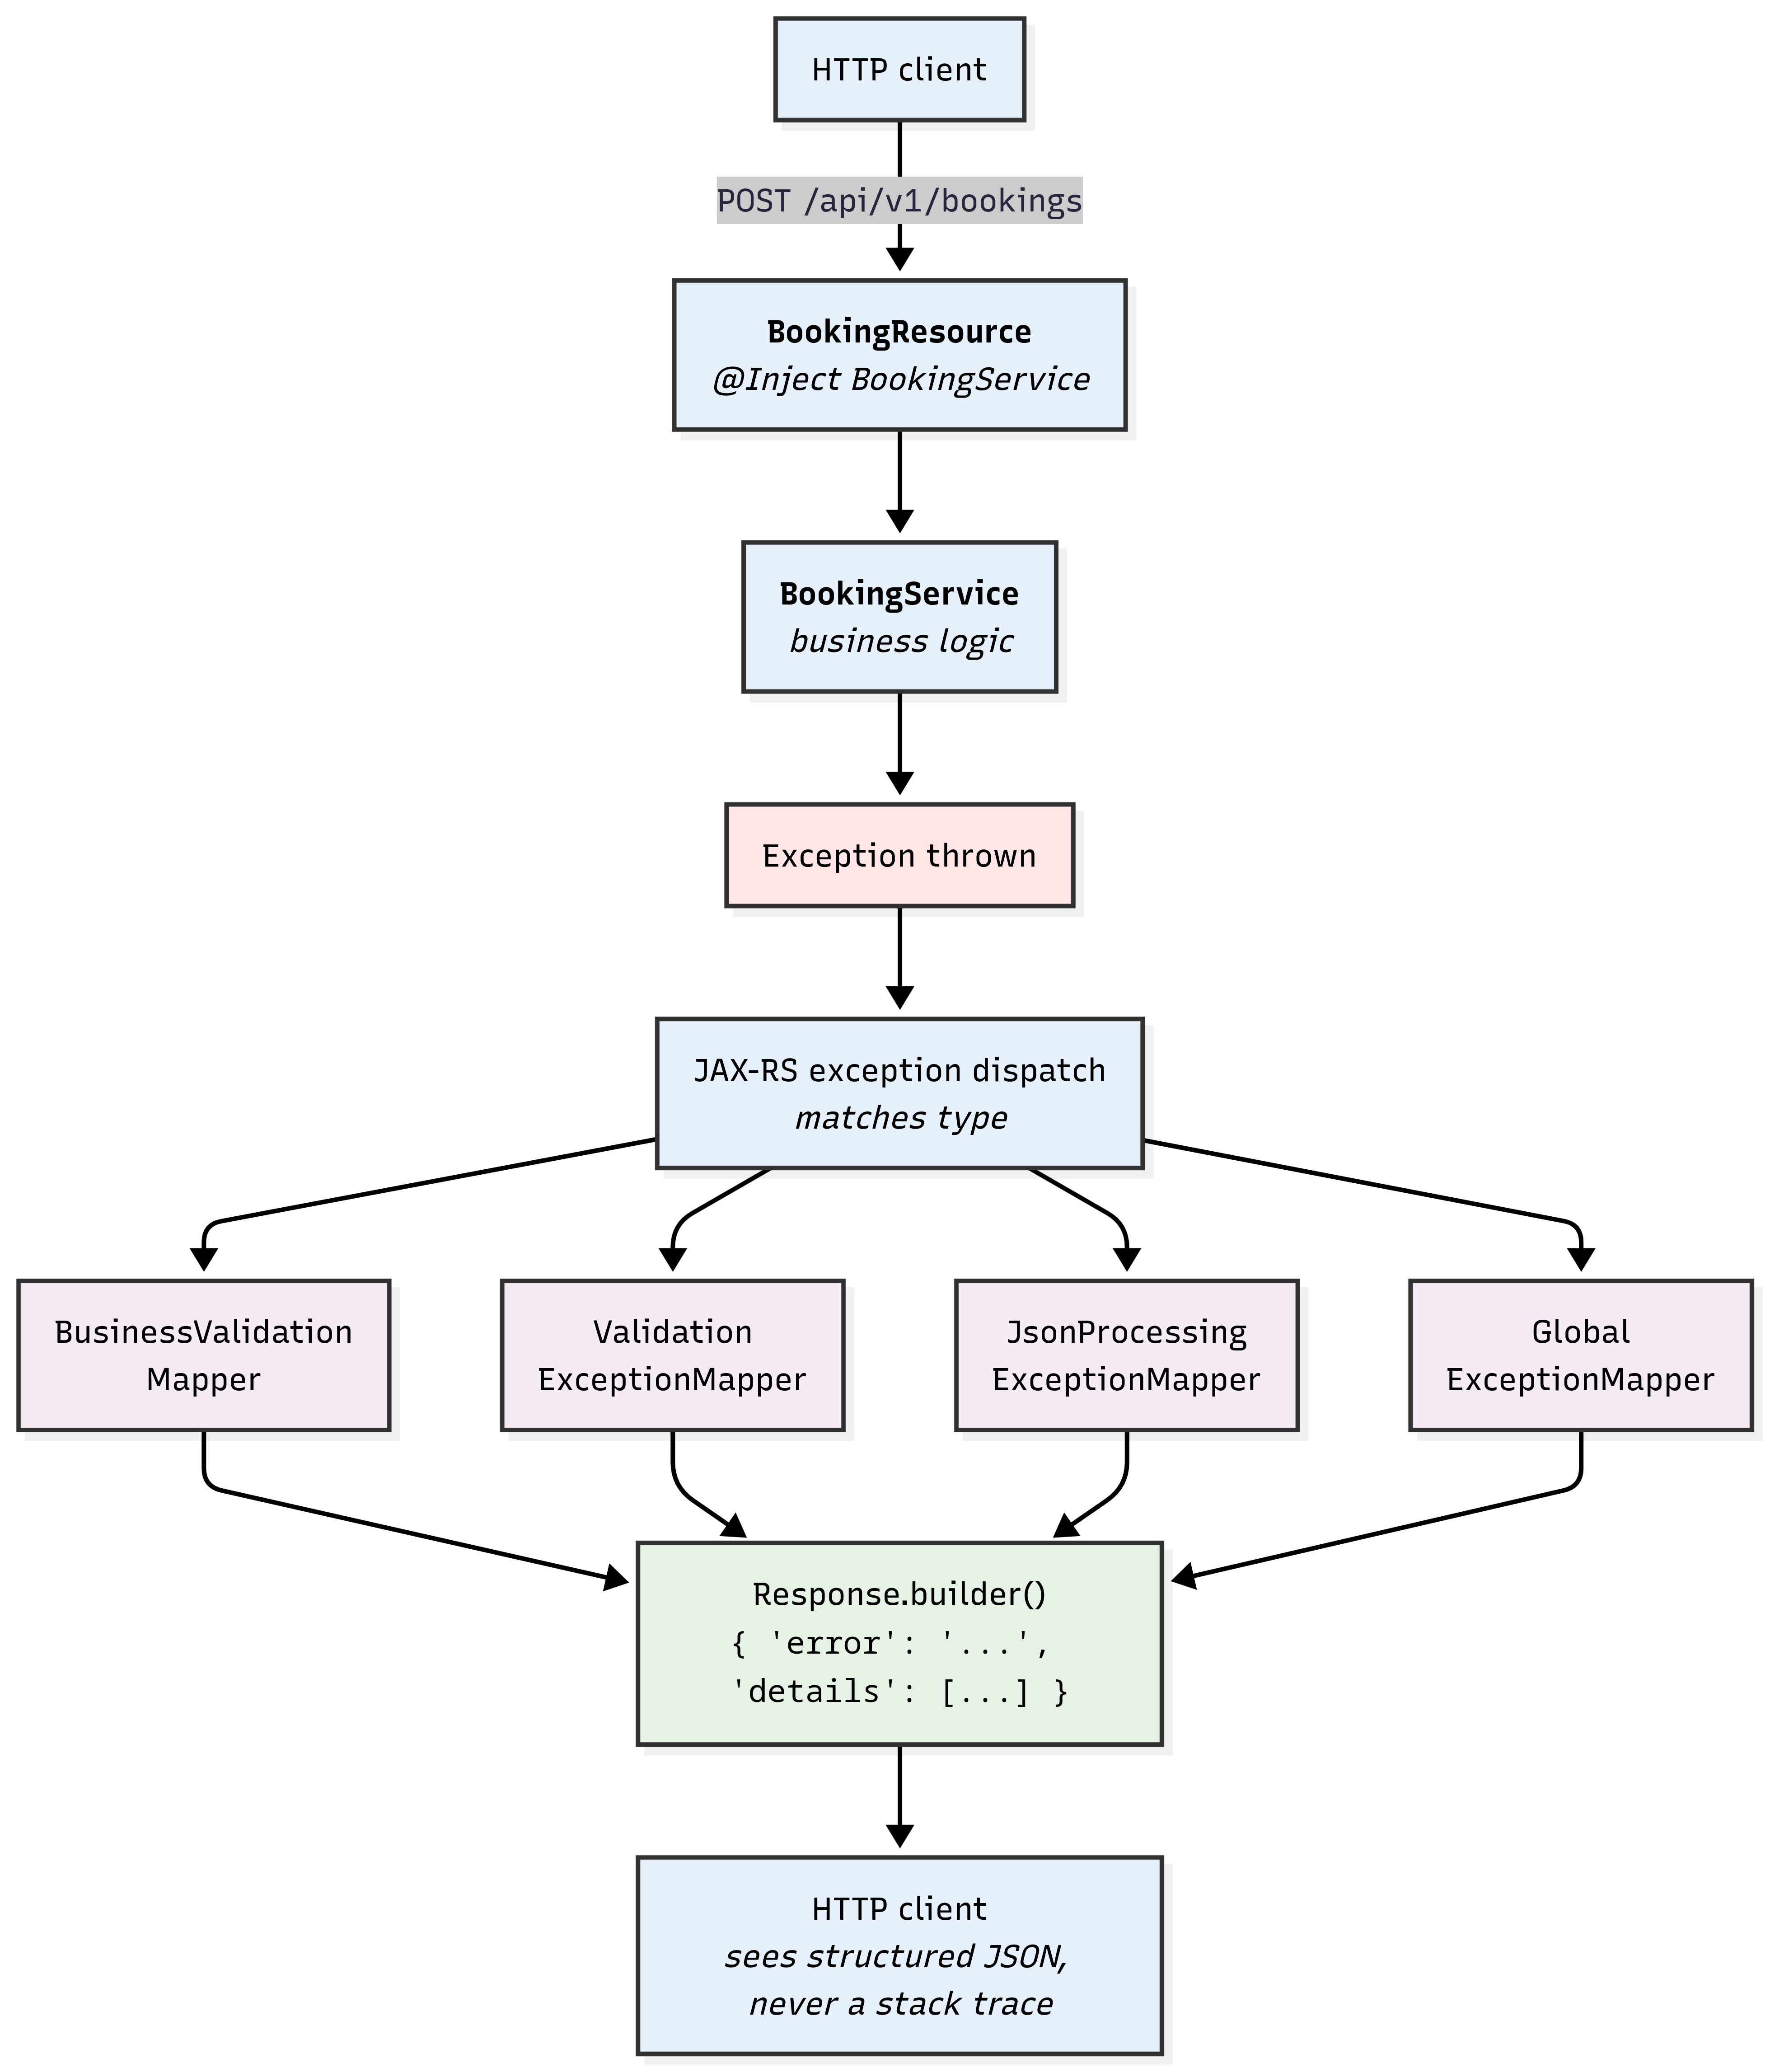
\includegraphics[width=\textwidth, height=14cm, keepaspectratio]{
		diagrams/syncspace-diagram.png
	}
	\caption{The \ac{CDI} + \ac{JAX-RS} exception-handling flow \ac{JSON} error
	body.}
	\label{fig:errormapper}
\end{figure}

Two patterns from \texttt{syncspace-jakarta-app} were adopted by the production
refactor: the use of a small set of focused \texttt{ExceptionMapper}s (which
keeps \ac{HTTP} status codes meaningful and gives the differential harness
a stable signal to assert on) and the use of \texttt{record}-based \acp{POJO}
for request and response bodies (which simplifies diffing). The remaining
features, in particular the full \ac{JWT} flow, were retained in the prototype
as a self-contained reference example for future students.

\section{Architecture of the Differential Testing Framework}
\label{sec:arch}

The architecture of the final testing framework, applied to the production \ac{API},
is summarised in Figure~\ref{fig:arch}. It is made of three concentric
layers: the GitLab pipeline, the harness processes, and the application instances
themselves.

\begin{figure}[H]
	\centering
	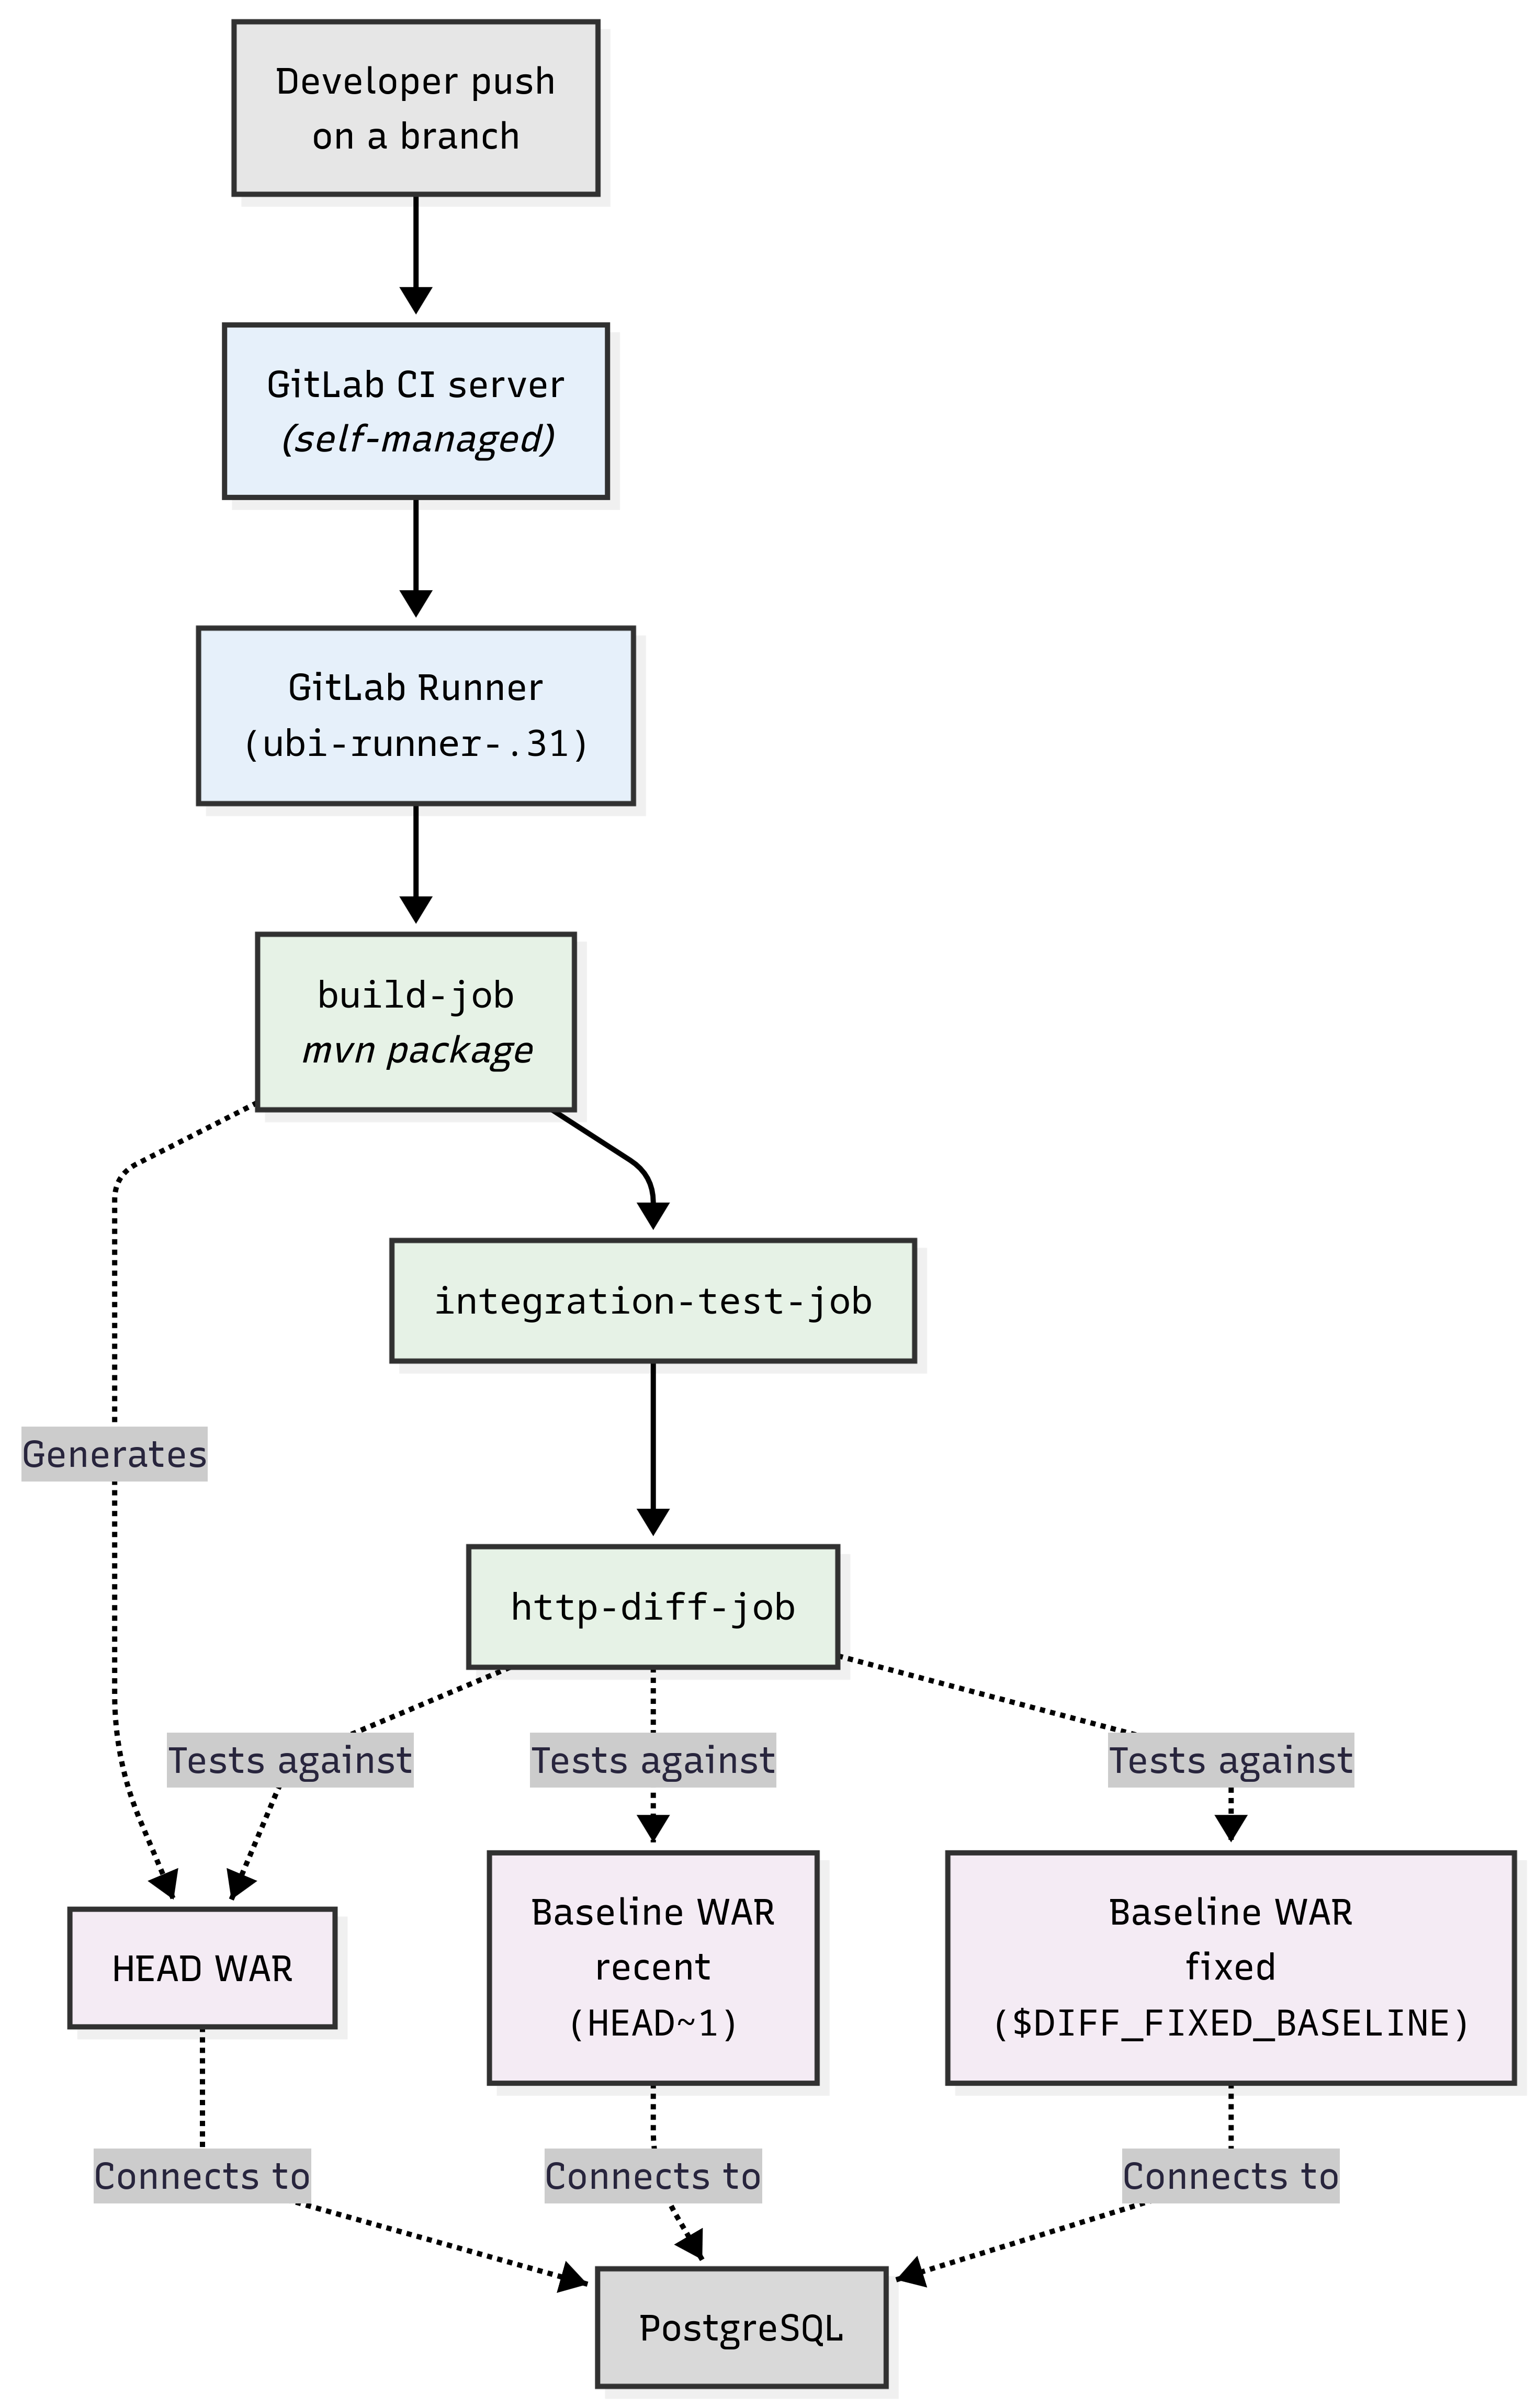
\includegraphics[width=\textwidth, height=14cm, keepaspectratio]{
		diagrams/ci-cd.png
	}
	\caption{Overall architecture of the differential testing framework.}
	\label{fig:arch}
\end{figure}

As illustrated, solid arrows denote execution flow, while dashed arrows
indicate artifact and data access. A developer push triggers a three-stage pipeline
on the internal runner (\texttt{ubi-runner-.31}):

First, \texttt{build-job} compiles the candidate \texttt{HEAD} \ac{WAR}. Second,
\texttt{integration-test-job} executes the standard JUnit suite. Finally, the
core \texttt{http-diff-job} performs a three-way comparison. It uses Git worktrees
to reconstruct both the immediate parent and a fixed reference baseline,
boots all three \acp{WAR} simultaneously on independent Payara Micro ports,
and replays \texttt{http-diff-cases.json} against a shared database fixture.
The resulting diff reports are then collected by GitLab as test artifacts.

Having refined this architecture through earlier prototypes---which traded
execution speed for a stricter separation of concerns---the next chapter
details the framework's application to the production \ac{API}.